\section{Introducción}

Una red de $N$ nodos entrena de forma colaborativa un modelo durante varias rondas, sin compartir datos crudos. Cada actualización se protege con ruido calibrado: más ruido protege más, pero reduce la utilidad de la actualización. En cada ronda hay que tomar dos decisiones:
\begin{enumerate}
  \item \textbf{Selección:} qué subconjunto de nodos participa.
  \item \textbf{Reparto:} cuánto del presupuesto de ruido se le asigna a cada nodo seleccionado.
\end{enumerate}

Este informe estudia la dificultad computacional de ambas decisiones. Se demuestra que:
\begin{itemize}
  \item el \textbf{reparto del presupuesto} (Parte 1) se resuelve de forma exacta en tiempo polinomial con un algoritmo voraz, cuya función de eficiencia es $\Theta(N + B\log N)$ en el peor caso;
  \item la \textbf{selección de participantes} (Parte 2) es \textbf{NP-difícil}, mediante una reducción desde \MC{}, de modo que no existe un algoritmo exacto de tiempo polinomial a menos que $\mathrm{P}=\mathrm{NP}$; por ello se usa un algoritmo voraz de aproximación con garantía $(1-1/e)$ y costo $\Theta(N\,k)$ evaluaciones.
\end{itemize}

\section{Preliminares}

\subsection{Notación asintótica}

Sean $T, g : \N \to \R_{\ge 0}$. Se usan las definiciones formales \parencite{cormen2009}:

\begin{definicion}[Cota superior, $O$]
$T(n) \in O(g(n))$ si existen constantes $c > 0$ y $n_0 \in \N$ tales que $T(n) \le c\, g(n)$ para todo $n \ge n_0$.
\end{definicion}

\begin{definicion}[Cota inferior, $\Omega$]
$T(n) \in \Omega(g(n))$ si existen constantes $c > 0$ y $n_0 \in \N$ tales que $T(n) \ge c\, g(n)$ para todo $n \ge n_0$.
\end{definicion}

\begin{definicion}[Cota ajustada, $\Theta$]
$T(n) \in \Theta(g(n))$ si $T(n) \in O(g(n))$ y $T(n) \in \Omega(g(n))$; es decir, existen $c_1, c_2 > 0$ y $n_0$ tales que $c_1 g(n) \le T(n) \le c_2 g(n)$ para todo $n \ge n_0$.
\end{definicion}

\begin{observacion}[Peor caso, mejor caso y cota del algoritmo]\label{obs:casos}
Cuando el número de operaciones depende de los datos (no solo del tamaño), se distinguen $T_{\text{peor}}(n)$ y $T_{\text{mejor}}(n)$. En ese caso se reporta: $T(n)\in O(T_{\text{peor}})$, $T(n)\in\Omega(T_{\text{mejor}})$, y una cota $\Theta$ para cada caso por separado. Cuando el algoritmo realiza siempre las mismas operaciones para un tamaño dado, $T_{\text{peor}} = T_{\text{mejor}}$ y el algoritmo tiene una única cota $\Theta$.
\end{observacion}

\subsection{Modelo de costo}

Se usa el modelo RAM: las operaciones aritméticas, comparaciones, asignaciones y accesos a arreglos cuestan tiempo constante. Para la Parte 2 la utilidad conjunta $f$ se consulta como una función; el costo de una evaluación de $f$ se denota $\tau$ (como en el enunciado) y se reporta por separado, de modo que el costo total se expresa como (número de evaluaciones)$\,\times \tau$.

\subsection{Problemas de decisión, P, NP y reducciones}

Las clases P y NP se definen sobre \textbf{problemas de decisión}, cuya respuesta es \emph{sí} o \emph{no}. Un problema de optimización (``maximizar $f$'') se convierte en uno de decisión agregando un umbral $t$ (``¿existe una solución con valor $\ge t$?'').

\begin{definicion}[Reducción polinomial]
Un problema $A$ se \emph{reduce polinomialmente} a un problema $B$, y se escribe $A \le_p B$, si existe una función $\varphi$, calculable en tiempo polinomial, que transforma cada instancia $I$ de $A$ en una instancia $\varphi(I)$ de $B$ tal que
\[
I \text{ tiene respuesta \emph{sí} en } A \iff \varphi(I) \text{ tiene respuesta \emph{sí} en } B.
\]
\end{definicion}

\begin{definicion}[NP-difícil y NP-completo]
Un problema $B$ es \emph{NP-difícil} si todo problema de NP se reduce polinomialmente a $B$. Es \emph{NP-completo} si además $B \in \mathrm{NP}$.
\end{definicion}

\begin{teorema}[Herramienta de la reducción]\label{teo:herramienta}
Si $A$ es NP-difícil y $A \le_p B$, entonces $B$ es NP-difícil.
\end{teorema}
\begin{proof}
Sea $X \in \mathrm{NP}$. Como $A$ es NP-difícil, existe $\varphi_1$ polinomial con $X \le_p A$. Por hipótesis existe $\varphi_2$ polinomial con $A \le_p B$. La composición $\varphi_2 \circ \varphi_1$ es polinomial (la composición de polinomios es un polinomio) y conserva la respuesta, porque cada transformación la conserva. Así $X \le_p B$ para todo $X\in\mathrm{NP}$.
\end{proof}

\begin{observacion}[Dirección de la reducción]
Para demostrar que \emph{nuestro} problema $B$ es difícil, la reducción va \textbf{desde} un problema $A$ ya conocido como difícil \textbf{hacia} $B$. La interpretación es: si existiera un algoritmo polinomial para $B$, se podría resolver $A$ en tiempo polinomial transformando sus instancias con $\varphi$. Reducir en la dirección contraria ($B \le_p A$) solo mostraría que $B$ \emph{no es más difícil} que $A$, lo cual no aporta nada.
\end{observacion}

\subsection{El conjunto potencia \texorpdfstring{$\pot{V}$}{2\^{}V}}

Para un conjunto finito $V$, $\pot{V}$ denota el \emph{conjunto potencia}: el conjunto de \textbf{todos} los subconjuntos de $V$. Una función de la forma $f:\pot{V}\to\R_{\ge 0}$ recibe un \emph{subconjunto} de $V$ y devuelve un número.

\begin{lema}\label{lem:potencia}
Si $|V| = N$, entonces $|\pot{V}| = 2^N$ y $\displaystyle\sum_{k=0}^{N}\binom{N}{k} = 2^N$.
\end{lema}
\begin{proof}
Para formar un subconjunto, cada uno de los $N$ elementos tiene dos opciones independientes: pertenecer o no pertenecer. Por el principio multiplicativo hay $2\cdot 2\cdots 2 = 2^N$ subconjuntos. Agrupándolos por tamaño, hay exactamente $\binom{N}{k}$ subconjuntos de tamaño $k$, y al sumar sobre $k=0,\dots,N$ se cuenta cada subconjunto una sola vez.
\end{proof}

La Figura~\ref{fig:arbol} muestra los subconjuntos de $V=\{1,2,3\}$ organizados en un árbol: a cada nodo solo se le agregan elementos mayores que su máximo, por lo que ningún subconjunto se repite. El nivel $k$ del árbol contiene los $\binom{3}{k}$ subconjuntos de tamaño $k$, que son exactamente los candidatos del problema de selección con cupo $k$.

\begin{figure}[H]
\centering
\begin{tikzpicture}[
  every node/.style={circle,draw,thick,minimum size=9mm,inner sep=1pt,font=\small},
  level distance=13mm]
  \node (e) at (0,0) {$\emptyset$};
  \node (1) at (2.4, 1.3) {$1$};
  \node (2) at (2.4, 0)   {$2$};
  \node (3) at (2.4,-1.3) {$3$};
  \node (12) at (4.8, 2.0) {$1,2$};
  \node (13) at (4.8, 0.8) {$1,3$};
  \node (23) at (4.8,-0.4) {$2,3$};
  \node (123) at (7.2, 2.0) {\scriptsize $1,2,3$};
  \draw (e)--(1); \draw (e)--(2); \draw (e)--(3);
  \draw (1)--(12); \draw (1)--(13); \draw (2)--(23);
  \draw (12)--(123);
  \begin{scope}[every node/.style={font=\footnotesize}]
    \node at (0,-2.5)   {$\binom{3}{0}=1$};
    \node at (2.4,-2.5) {$\binom{3}{1}=3$};
    \node at (4.8,-2.5) {$\binom{3}{2}=3$};
    \node at (7.2,-2.5) {$\binom{3}{3}=1$};
  \end{scope}
\end{tikzpicture}
\caption{Árbol de los $2^3=8$ subconjuntos de $V=\{1,2,3\}$, agrupados por tamaño.}
\label{fig:arbol}
\end{figure}
